\section{Field Rest-Energy Records}\label{manual:rest-energy-prediction}

\subsection{0\texorpdfstring{$|-$}{|-} scope}\label{manual:rest:scope}
Rest-energy records are split into two tables. The A\(\Omega\) field-map table records support, carried cycle, and A\(\Omega\) accessor values. The measured-data comparison table records declared measured-sector target rows.
\[
\mathbf a\vdash(F,R,\partial_T R,\omega),
\qquad
B=(\partial_TF,\omega).
\]
The calculation spine is
\[
C_f[M]_{\AO}
\longrightarrow
\mathsf{AO}_{\mu}(C)
\longrightarrow
\SADARop_B(C)
\longrightarrow
\nu_{x,\AO}
\longrightarrow
E_{x,\mathrm{ext}}.
\]
\aodnoteblock{Data-support class}{Rest-energy records are exact internal A\(\Omega\) field records or O0 external-map comparisons, depending on the declared measured-sector target rows. Uncertainty is scoped to the external measured-sector target and value map, not to a simulation medium.}

\aodprovenance{main:app:ao-field-fractal-properties.}

\subsection{Support notation used by the calculation records}\label{manual:rest:support-notation}
The manual uses compact support notation only where the calculation needs it:
\[
D_i\Box D_j=\text{open-seat duon support},
\]
\[
D_i\mu D_j,
\qquad
\mu\in\{-1,0,+1\},
\qquad
=\text{resolved duon support},
\]
\[
E_2^0=\text{open-seat duon support},
\qquad
E_2^\pm=\text{duad / seated duon support}.
\]
The compact field supports are
\[
1{:}2{:}L=\text{Dimonon support},
\qquad
3{:}q{:}L=\text{Trion support}.
\]
Odd lengths are carried as odd-window route status between adjacent even support enclosures:
\[
L=2k+1
\quad\Rightarrow\quad
C_{2k}\leadsto L\leadsto C_{2k+2}.
\]
When this odd-window instability is retained as a route-status suffix, write \(K_{\mathrm{yro}}\). The suffix is not a support-enclosure name.

\aodprovenance{main:app:ao-field-fractal-properties.}


\subsection{A\texorpdfstring{$\Omega$}{Omega} field-map table}\label{manual:rest:ao-field-value-table}
The A\(\Omega\) field-map table lists the manual mapping from measured-sector names to A\(\Omega\) field supports. Field-support properties are not repeated here; they are listed in the main note, App.~J.

\begin{table}[H]
\centering
\scriptsize
\caption{A\(\Omega\) field-map table.}
\begin{tabularx}{\textwidth}{l l l l l l}
\toprule
\(x_{\mathrm{ext}}\) & external map & \(M_x\) & \(C_f[M_x]_{\AO}\) & \(\nu_{x,\AO}\) & comparison\\
\midrule
\(e^-\) & \(00|-\) Dimonhexon & \(1{:}2{:}6\) & \(C_f[1{:}2]_{\AO}\) & \(\nu_{e,\AO}\) & target declared\\
\(\mu^-\) & \(00|-\) Dimonocton & \(1{:}2{:}8\) & \(C_f[1{:}2]_{\AO}\) & \(\nu_{\mu,\AO}\) & target declared\\
\(\tau^-\) & \(00|-\) Dimonnanyro & \(1{:}2{:}9_{\mathrm{yro}}\) & \(C_f[1{:}2]_{\AO}\) & \(\nu_{\tau,\AO}\) & target declared\\
\(B^\pm\) & Ditrion debris map & \(3{:}2{:}6\) & \(C_f[3{:}2]_{\AO}\) & \(\nu_{B,\AO}\) & target declared\\
\(B^0\) & Ditrion debris map & \(3{:}2{:}6\) & \(C_f[3{:}2]_{\AO}\) & \(\nu_{B,\AO}\) & target declared\\
\(B_s^0\) & lifted Ditrion map & \(3{:}2{:}8\) & \(C_f[3{:}2]_{\AO}\) & \(\nu_{B_s,\AO}\) & target declared\\
\(B_c^\pm\) & lifted Ditrion map & \(3{:}2{:}10\) & \(C_f[3{:}2]_{\AO}\) & \(\nu_{B_c,\AO}\) & target declared\\
\(p^+\) & Tritriohexon map & \(3{:}3{:}6\) & \(C_f[3{:}3]_{\AO}\) & \(\nu_{p,\AO}\) & target declared\\
\(n^0\) & Tetratriohexon map & \(3{:}4{:}6\) & \(C_f[3{:}4]_{\AO}\) & \(\nu_{n,\AO}\) & target declared\\
\bottomrule
\end{tabularx}
\label{tab:manual-ao-field-value-table}
\end{table}

\aodprovenance{main:app:ao-field-fractal-properties; main:subsec:curling-curl-support-forms.}
\aodremark{The manual declares measured-sector maps such as \(e^-\mapsto 00|-\) Dimonhexon. These maps are carried by manual comparison records; the main note lists the A\(\Omega\) field-property table.}

\subsection{Electron external map}\label{manual:rest:electron-external-map}
The electron comparison record is a manual map from the measured-sector electron to the A\(\Omega\) Dimonhexon support:
\[
e^-
\longmapsto
00|-\;\mathrm{Dimonhexon}
\equiv
00|-\;(1{:}2{:}6),
\qquad
C_f[1{:}2]_{\AO}.
\]
The charge-orientation tag is
\[
q_{\mathrm{ext}}(e^-)=-1,
\qquad
Q_{\mathrm{ext}}(e^-)=-e.
\]
The rest-energy comparison target remains quarantined:
\[
E^{\mathrm{tar}}_e=0.51099895069\ \mathrm{MeV},
\qquad
\sigma_{E,e}=1.6\times10^{-10}\ \mathrm{MeV}.
\]
\aodliteraturenote{Electron mass-energy: NIST CODATA~\cite{nist-electron-mass-energy}, SI defining constants: BIPM~\cite{bipm-si-defining-constants}.}
\aodremark{The \(00|-\) tag is a manual measured-sector charge/orientation map carried by the manual comparison record.}

\subsection{Measured-data comparison analysis}\label{manual:rest:measured-comparison-analysis}
External comparison is quarantined. For records with declared targets,
\[
E_{x,\mathrm{ext}}=K_{\mathrm{ext}}\nu_{x,\AO},
\qquad
\Delta E_x=E_{x,\mathrm{ext}}-E_x^{\mathrm{tar}},
\]
\[
\epsilon_x^{\mathrm{sgn}}
=
100\frac{\Delta E_x}{E_x^{\mathrm{tar}}},
\qquad
|\epsilon_x|=|\epsilon_x^{\mathrm{sgn}}|,
\qquad
z_x=\frac{\Delta E_x}{\sigma_{E,x}}.
\]

\begin{table}[H]
\centering
\scriptsize
\caption{Measured-data comparison analysis.}
\begin{tabularx}{\textwidth}{l c c c c c c l}
\toprule
\(x\) & \(E_{x,\mathrm{tar}}\) [MeV] & \(\sigma_{E,x}\) [MeV] & \(E_{x,\mathrm{ext}}\) & \(\Delta E_x\) & \(\epsilon_x\) & \(z_x\) & status\\
\midrule
\(e\) & 0.51099895069 & \(1.6\times10^{-10}\) & \(K_{\mathrm{ext}}\nu_{e,\AO}\) & formula & formula & formula & target declared\\
\(\mu\) & 105.6583755 & \(2.3\times10^{-6}\) & \(K_{\mathrm{ext}}\nu_{\mu,\AO}\) & formula & formula & formula & target declared\\
\(\tau\) & 1776.86 & 0.12 & \(K_{\mathrm{ext}}\nu_{\tau,\AO}\) & formula & formula & formula & target declared\\
\(B^\pm\) & 5279.41 & 0.07 & \(K_{\mathrm{ext}}\nu_{B,\AO}\) & formula & formula & formula & target declared\\
\(B^0\) & 5279.72 & 0.08 & \(K_{\mathrm{ext}}\nu_{B,\AO}\) & formula & formula & formula & target declared\\
\(B_s^0\) & 5366.93 & 0.10 & \(K_{\mathrm{ext}}\nu_{B_s,\AO}\) & formula & formula & formula & target declared\\
\(B_c^\pm\) & 6274.47 & 0.32 & \(K_{\mathrm{ext}}\nu_{B_c,\AO}\) & formula & formula & formula & target declared\\
\(p\) & 938.27208943 & \(2.9\times10^{-7}\) & \(K_{\mathrm{ext}}\nu_{p,\AO}\) & formula & formula & formula & target declared\\
\(n\) & 939.56542194 & \(4.8\times10^{-7}\) & \(K_{\mathrm{ext}}\nu_{n,\AO}\) & formula & formula & formula & target declared\\
\bottomrule
\end{tabularx}
\label{tab:manual-measured-comparison-analysis}
\end{table}

\aodprovenance{main:app:ao-field-fractal-properties; manual \appref{manual:external-comparison}.}

\aodliteraturenote{Lepton/baryon targets: NIST CODATA~\cite{nist-electron-mass-energy,nist-muon-mass-energy,nist-tau-mass-energy,nist-proton-mass-energy,nist-neutron-mass-energy}, meson targets: PDG 2025~\cite{pdg-bmeson-2025}.}

\subsection{Tritrioseptyro Higgs-support diagnostic fixture}\label{manual:tritrioseptyro-higgs-support-fixture}
Tritrioseptyro is the \(3{:}3{:}7_{\mathrm{yro}}\) Higgs-support prediction candidate selected by the internal AFC trace. The AFC run produces the trace rows; A\(\Omega\) detectors read the trace and name the retained route status. The selected candidate is joined to the frozen external mass map \(E_H=RD\,2^{L+4}\) MeV. Production-channel and decay-channel residual tables carry the next comparison layer.
\[
\text{AFC run}\longrightarrow \text{read-only trace}\longrightarrow \text{A\(\Omega\) route-status naming}.
\]
The trace is read-only unless a feedback experiment is explicitly declared.

The candidate set is
\[
\mathcal K_H=
\{3{:}1{:}7,3{:}1{:}9,3{:}2{:}7,3{:}2{:}9,
3{:}3{:}7,3{:}3{:}9,3{:}4{:}7,3{:}4{:}9\}.
\]
For each candidate \(K=(p,q,L)\), compute
\[
\Pi=q^p+q,
\qquad
RD=2\Pi+1,
\qquad
\rho^D_\omega=\min(RD,L).
\]
The scoped collision capacity is
\[
C_{3,H}=3.
\]
With this scoped collision capacity,
\[
P^D_H=C_{3,H}\rho^D_\omega,
\qquad
Q^D_H=C_{3,H}\max(0,RD-L).
\]
The retained candidate is
\[
K_H^\star=3{:}3{:}7_{\mathrm{yro}}=\mathrm{Tritrioseptyro}.
\]
For Tritrioseptyro,
\[
\Pi=30,
\qquad
RD=61,
\qquad
\rho^D_\omega=7,
\qquad
P^D_H=21,
\qquad
Q^D_H=162.
\]
Against adjacent even support-enclosure closures,
\[
P^D_H-C_6=+3,
\qquad
P^D_H-C_8=-3.
\]
The trace places Tritrioseptyro on the \(C_6/C_8\) saddle with pressure residuals \(+3\) and \(-3\) and pending overhang \(Q^D_H=162\).

\begin{table}[H]
\centering
\scriptsize
\caption{Internal Higgs-support candidates. This table carries AFC trace quantities for candidate selection. External comparison columns are carried by the frozen-map comparison table.}
\begin{tabular}{lrrrrrrr}
\toprule
Candidate & \(\Pi\) & \(RD\) & \(\rho^D_\omega\) & \(P^D_H\) & \(Q^D_H\) & saddle & score \\
\midrule
\(3{:}3{:}7_{\mathrm{yro}}\) & 30 & 61 & 7 & 21 & 162 & \(+3/-3\) & 0.00 \\
\(3{:}2{:}7_{\mathrm{yro}}\) & 10 & 21 & 7 & 21 & 42 & \(+3/-3\) & 1.58 \\
\(3{:}3{:}9_{\mathrm{yro}}\) & 30 & 61 & 9 & 27 & 156 & \(+3/0\) & 2.25 \\
\(3{:}4{:}7_{\mathrm{yro}}\) & 68 & 137 & 7 & 21 & 390 & \(+3/-3\) & 2.40 \\
\(3{:}2{:}9_{\mathrm{yro}}\) & 10 & 21 & 9 & 27 & 36 & \(+3/0\) & 2.89 \\
\(3{:}1{:}7_{\mathrm{yro}}\) & 2 & 5 & 5 & 15 & 0 & \(-3/-9\) & 3.00 \\
\(3{:}4{:}9_{\mathrm{yro}}\) & 68 & 137 & 9 & 27 & 384 & \(+3/0\) & 3.59 \\
\(3{:}1{:}9_{\mathrm{yro}}\) & 2 & 5 & 5 & 15 & 0 & \(-9/-12\) & 4.75 \\
\bottomrule
\end{tabular}
\label{tab:manual-higgs-internal-candidates}
\end{table}

The trace score is reproducible and contains no candidate-identity override:
\[
S_H(K)=\frac{d_{\mathrm{saddle}}}{12}+\frac{d_Q}{100}+\frac{d_L}{2}+d_{\mathrm{route}}.
\]
The scoring gate requires
\[
\arg\min_{K\in\mathcal K_H}S_H(K)=3{:}3{:}7_{\mathrm{yro}}.
\]

\begin{figure}[H]
\centering
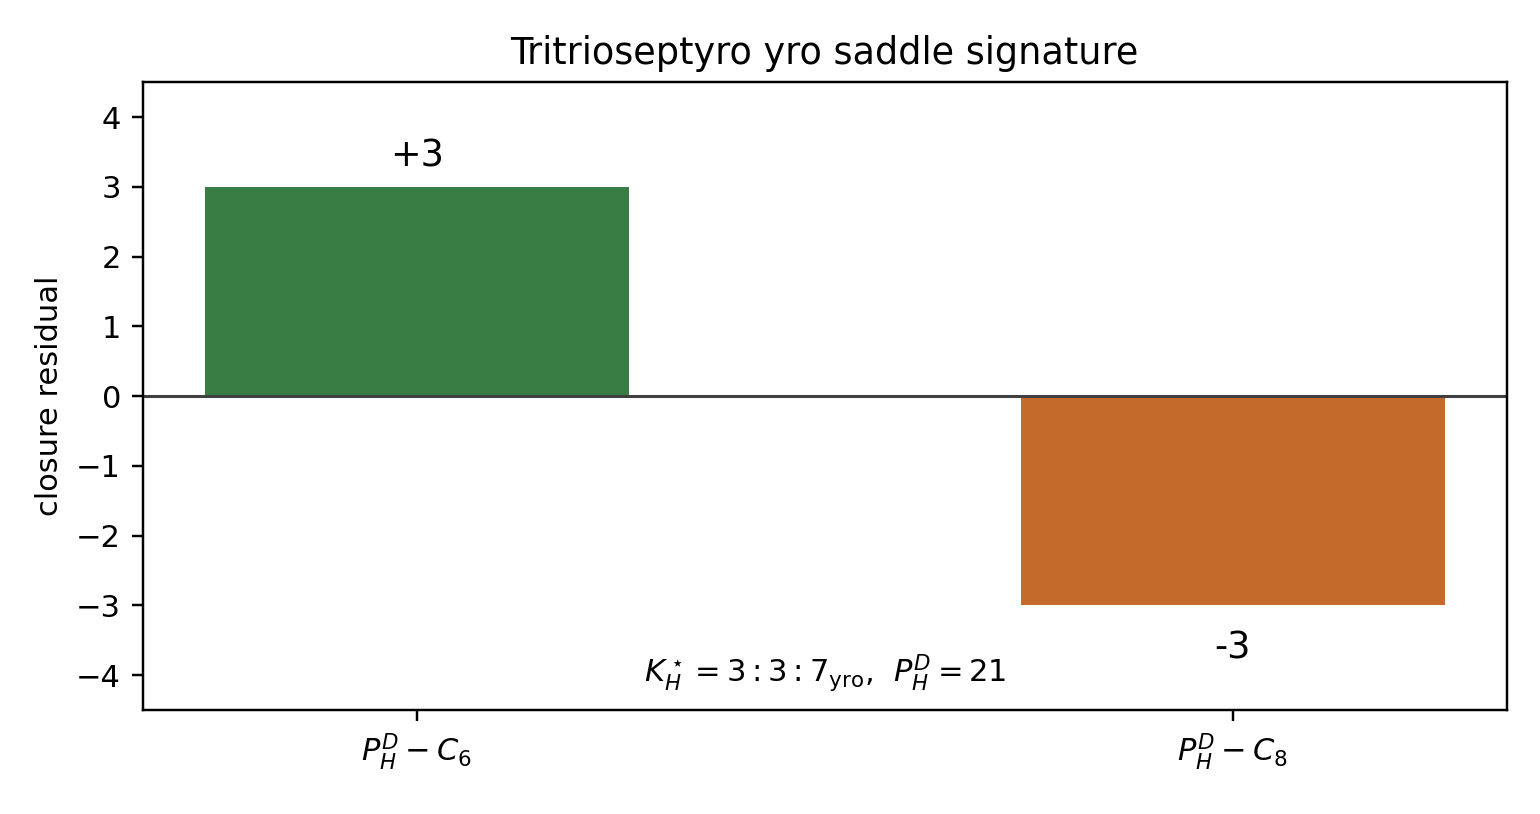
\includegraphics[width=0.72\linewidth]{figures/higgs/higgs_yro_saddle_signature.png}
\caption{Tritrioseptyro yro saddle signature. The internal AFC trace gives \(P^D_H=21\), placing the selected \(3{:}3{:}7_{\mathrm{yro}}\) candidate between \(C_6=18\) and \(C_8=24\) with residuals \(+3\) and \(-3\).}
\label{fig:manual-higgs-yro-saddle}
\end{figure}

\begin{figure}[H]
\centering
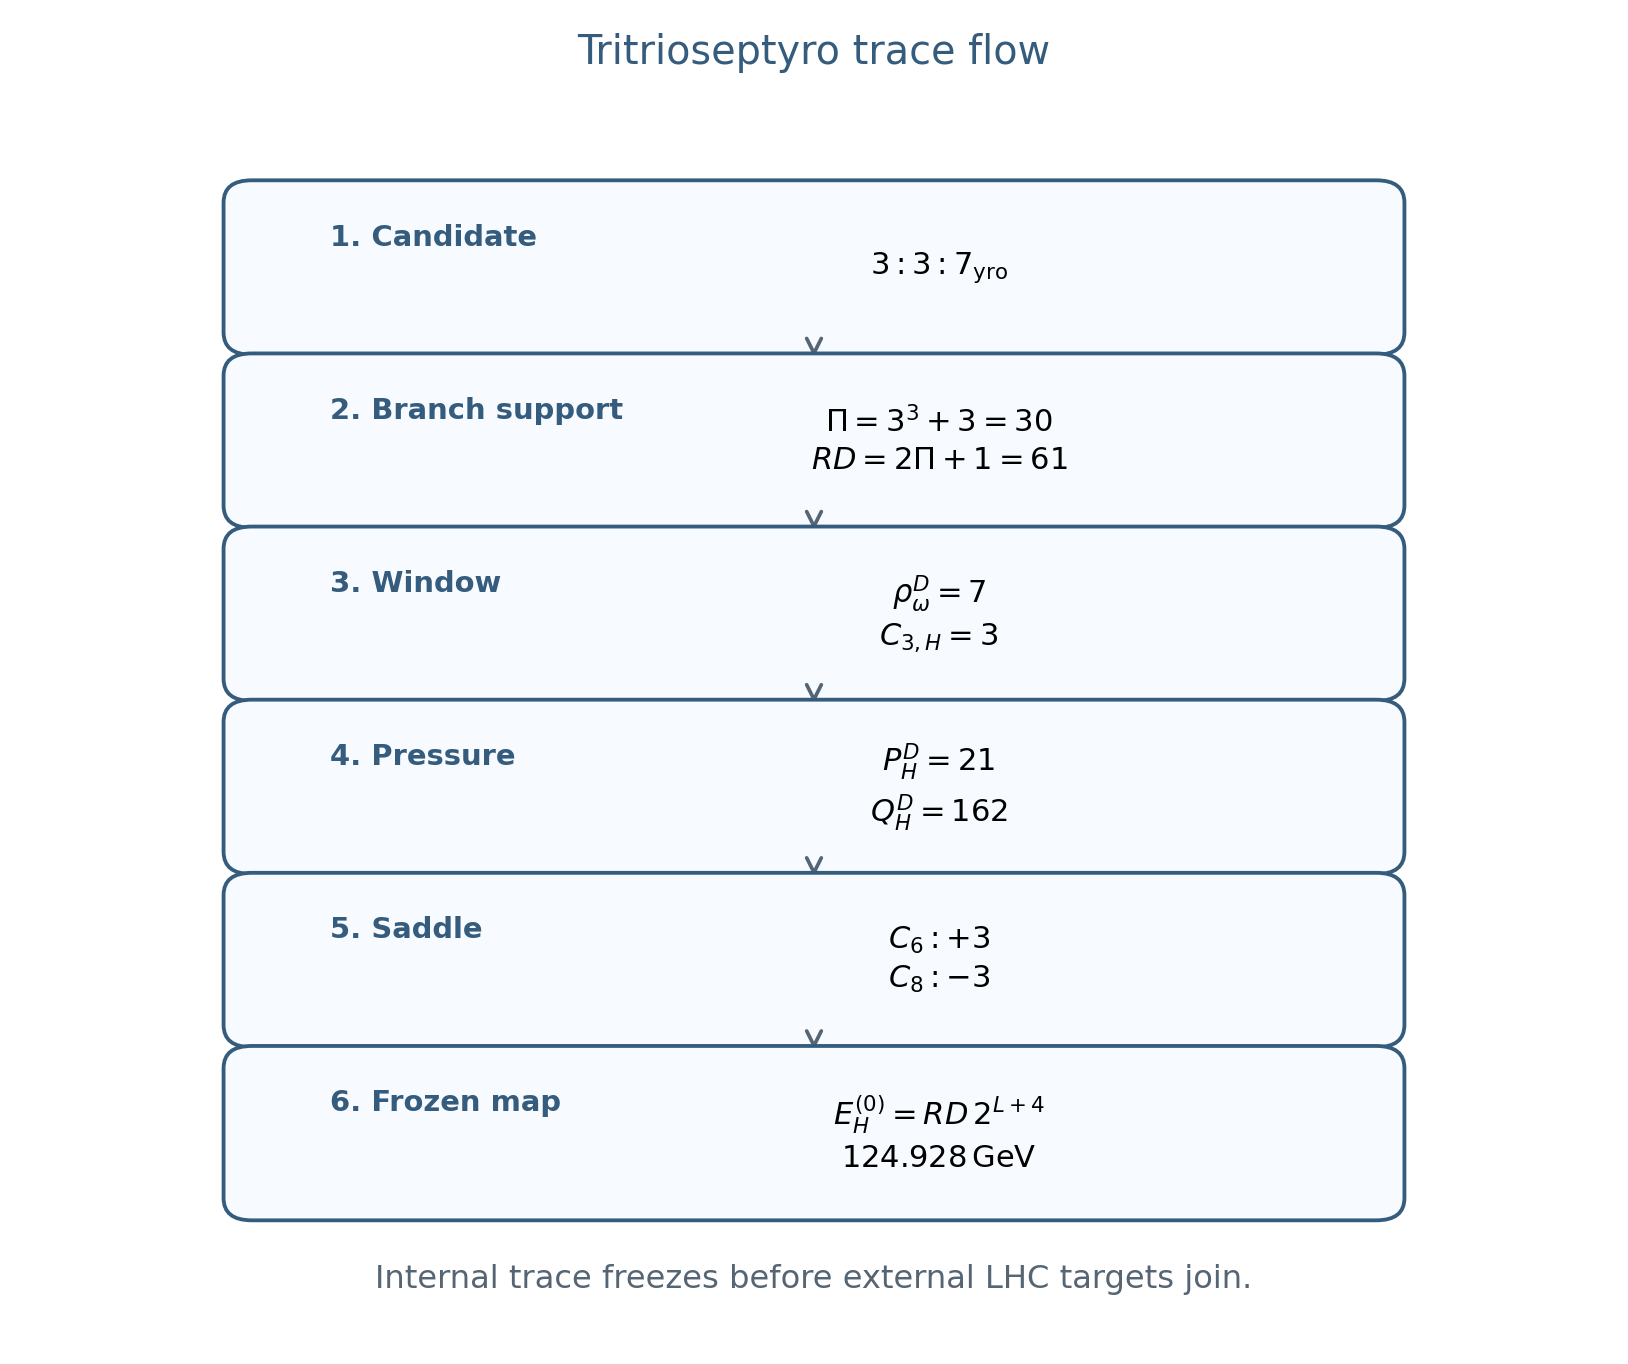
\includegraphics[width=0.92\linewidth]{figures/higgs/higgs_tritrioseptyro_trace_flow.png}
\caption{Tritrioseptyro trace flow. The AFC run produces \(\Pi=30\), \(RD=61\), \(\rho^D_\omega=7\), \(P^D_H=21\), and \(Q^D_H=162\). A\(\Omega\) names the detected \(3{:}3{:}7_{\mathrm{yro}}\) route status as Tritrioseptyro.}
\label{fig:manual-higgs-trace-flow}
\end{figure}

\subsubsection{External mass map after candidate freeze}\label{manual:higgs-external-map-after-freeze}
The external mass map is frozen after the internal candidate is selected:
\[
E_H^{(0)}[\mathrm{MeV}]=RD_H\,2^{L+4}.
\]
For Tritrioseptyro,
\[
E_H^{(0)}=61\cdot2^{11}\ \mathrm{MeV}=124928\ \mathrm{MeV}=124.928\ \mathrm{GeV}.
\]
The frozen \(RD\,2^{L+4}\) map sends Tritrioseptyro to \(124.928\,\mathrm{GeV}\). Declared Higgs mass targets enter after the candidate and external map are frozen. The comparison table reports \(\Delta E\), absolute percent error, and \(z\)-score for each target record.

\begin{table}[H]
\centering
\scriptsize
\caption{Frozen external map for Tritrioseptyro.}
\begin{tabular}{l l l}
\toprule
Quantity & Value & Status \\
\midrule
\(K_H^\star\) & \(3{:}3{:}7_{\mathrm{yro}}\) & frozen internal candidate \\
\(RD_H\) & 61 & frozen internal accessor \\
\(L\) & 7 & declared odd window \\
\(E_H^{(0)}\) & \(61\cdot2^{11}\,\mathrm{MeV}=124.928\,\mathrm{GeV}\) & external map after freeze \\
\bottomrule
\end{tabular}
\label{tab:manual-higgs-external-map}
\end{table}

\begin{table}[H]
\centering
\scriptsize
\caption{LHC mass comparison after frozen external map.}
\begin{tabular}{lrrrrr}
\toprule
Target & Mass [GeV] & \(\sigma\) [GeV] & \(\Delta E\) [GeV] & \(|\epsilon|\) [\%] & \(z\) \\
\midrule
ATLAS+CMS Run-1 combined & 125.09 & 0.24 & -0.162 & 0.1295 & -0.675 \\
CMS \(H\to4\ell\) & 125.04 & 0.12 & -0.112 & 0.0896 & -0.933 \\
ATLAS Run-1+2 combined & 125.11 & 0.11 & -0.182 & 0.1455 & -1.655 \\
ATLAS \(H\to\gamma\gamma\) & 125.22 & 0.14 & -0.292 & 0.2332 & -2.086 \\
\bottomrule
\end{tabular}
\label{tab:manual-higgs-lhc-comparison}
\end{table}

\begin{figure}[H]
\centering
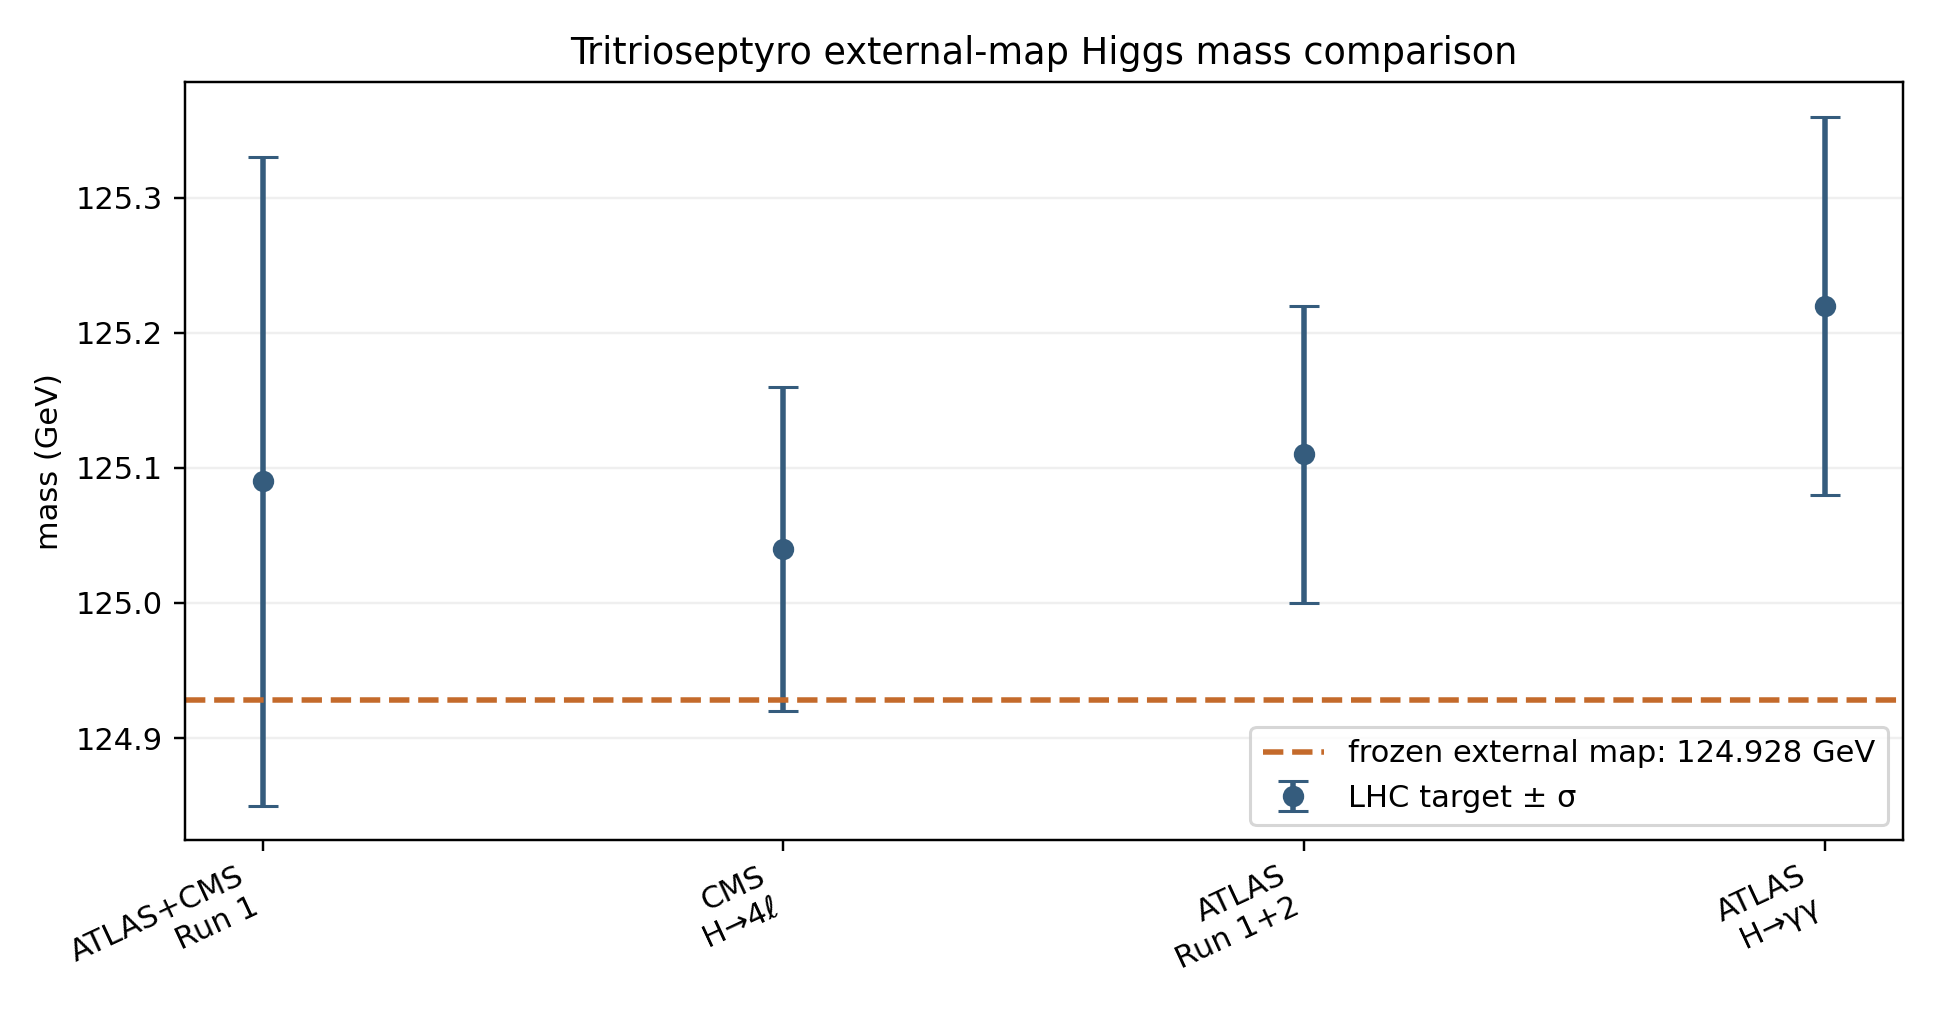
\includegraphics[width=0.88\linewidth]{figures/higgs/higgs_mass_comparison.png}
\caption{Tritrioseptyro mass comparison. The frozen external map \(E_H=RD\,2^{L+4}\) MeV sends the selected candidate to \(124.928\,\mathrm{GeV}\). Target records enter as declared external comparison rows.}
\label{fig:manual-higgs-mass-comparison}
\end{figure}

\paragraph{External data-comparison record.}
The internal trace selects \(K^\star_H=3{:}3{:}7_{\mathrm{yro}}\). The frozen external map gives
\[
E_H^{(0)}=RD_H2^{L+4}=61\cdot2^{11}\,\mathrm{MeV}=124.928\,\mathrm{GeV}.
\]
Table~\ref{tab:manual-higgs-lhc-comparison} records the declared Higgs mass-input rows, their quoted uncertainties, and the resulting \(\Delta E\), \(|\epsilon|\), and \(z\) coordinates. The mapped value \(124.928\,\mathrm{GeV}\) lies within \(1\sigma\) of the ATLAS+CMS Run-1 combined mass record and the CMS Run-2 \(H\to4\ell\) mass record. Production-channel and decay-channel residual tables carry the next comparison layer.

\aodliteraturenote{ATLAS+CMS Run-1 combined mass~\cite{atlas-cms-higgs-run1}. CMS \(H\to4\ell\) mass~\cite{cms-hig-21-019}. ATLAS combined Run-1+Run-2 mass~\cite{atlas-higgs-mass-combined-2023}. ATLAS diphoton mass~\cite{atlas-higgs-diphoton-2023}.}
\aodprovenance{main:subsec:yro-odd-window-route-status; main:app:ao-field-fractal-properties; manual:tab:manual-higgs-internal-candidates; manual:tab:manual-higgs-external-map.}

